
\documentclass[a4paper,12pt,titlepage,finall]{article}

\usepackage{amsmath}
\usepackage{amsfonts}
\usepackage{amssymb}\usepackage{amssymb}
\usepackage{csvsimple}
\usepackage{tikz}
\usepackage{pgfplots}
\usepackage{cmap}
\usepackage{color}
\usepackage[utf8x]{inputenc}
\usepackage[english,russian]{babel}
\usepackage[T2A]{fontenc}
\newcommand{\gt}{\textgreater} % знак больше
\newcommand{\lt}{\textless}       % знак меньше]
\usepackage[margin=2cm]{geometry}		 % для настройки размера полей
\usepackage{indentfirst}         % для отступа в первом абзаце секции
\usepackage{amsmath}
\usepackage{fancyvrb}
\usepackage{listings}
\usepackage{algorithm}
\usepackage{algpseudocode}
\usepackage{bm}
\usepackage{hyperref}

\usepackage{csvsimple}

\pgfplotsset{compat=1.11}
\usetikzlibrary{calc}
\lstset{
	inputencoding=utf8x,
	extendedchars=false,
	keepspaces = true,
	language=C++,
	basicstyle=\ttfamily,
	keywordstyle=\color[rgb]{0,0,1},
	stringstyle=\color[rgb]{0.627,0.126,0.941},
	numberstyle=\color[rgb]{0.205, 0.142, 0.73},
	frame=shadowbox,
	escapechar=`,
	numbers=left,
	breaklines=true,
	basicstyle=\ttfamily,
	literate={\ \ }{{\ }}1,
	tabsize=2,
	basicstyle=\footnotesize,
}
\lstset{language=C++,
	basicstyle=\ttfamily,
	keywordstyle=\color{blue}\ttfamily,
	stringstyle=\color{red}\ttfamily,
	%commentstyle=\color{green}\ttfamily,
	%morecomment=[l][\color{magenta}]{\#}
}
\DeclareMathOperator*{\EE}{\mathbb{E}}
\DeclareMathOperator*{\PP}{\mathbb{P}}
% выбираем размер листа А4, все поля ставим по 2см
\geometry{a4paper,left=20mm,top=20mm,bottom=20mm,right=20mm}

\setcounter{secnumdepth}{0}      % отключаем нумерацию секций

\begin{document}
	% Титульный лист
	\begin{titlepage}
		\begin{center}
			{\small \sc Московский государственный университет \\имени М.~В.~Ломоносова\\
				Факультет вычислительной математики и кибернетики\\
				Кафедра математических методов прогнозирования}
			\vfill
			{\Large \sc Отчёт по заданию 3. \\ Ансамбли алгоритмов. Веб-сервер. \\ Композиции алгоритмов для решения задачи регрессии.}\\
		\end{center}
		\begin{flushright}
			\vfill {Выполнила:\\
				Пронина Наталия\\
				317 группа\\
				~\\}
		\end{flushright}
		\begin{center}
			\vfill
			{\small Москва\\2021}
		\end{center}
	\end{titlepage}
		
% Автоматически генерируем оглавление на отдельной странице
\tableofcontents
\newpage


\begin{section}{Введение}
    В данном отчёте представлено описание экспериментов, которые были направлены на исследование двух моделей ансамблирования решающих деревьев: случайный лес (RF) и градиентный бустинг (GB).
    Эксперименты проводились на датасете с данными о недвижимости (House Sales in King County, USA). \par Цель: предсказать цену недвижимости
    
    Рассматривается задача регрессии с метрикой качества
  $ RMSE = \sqrt{\frac{1}{N} \sum_{i=1}^{N} (y_i - a_i)^2  } $ ,  где $N$~--- размер выборки, $y_i$~--- истинное значение целевой переменной на $i$-м объекте, \\ $a_i$~--- предсказанное.

\end{section}


\begin{section}{Эксперименты}
	
\begin{subsection}{1) Предобработка текста}
В датасете имеется только один признак типа object - это дата. Разобьём этот признак на три целочисленных - число, месяц и год, в итоге получается 21 признак. Удалим признак <<id>>. Разделим выборку на обучающую и валидационную в отношении 7:3.
\end{subsection}

\begin{subsection}{2) Случайный лес}
Будем поочереди фиксировать лучшие найденные параметры и подбирать следующие. При исследовании зависимости от количества деревьев алгоритм обучался только один раз, так как в методе $fit$ все исследуемые величины сохраняются в отдельные массивы.

\begin{subsubsection}{2.1) Количество деревьев в ансамбле}
\begin{figure}[H]
	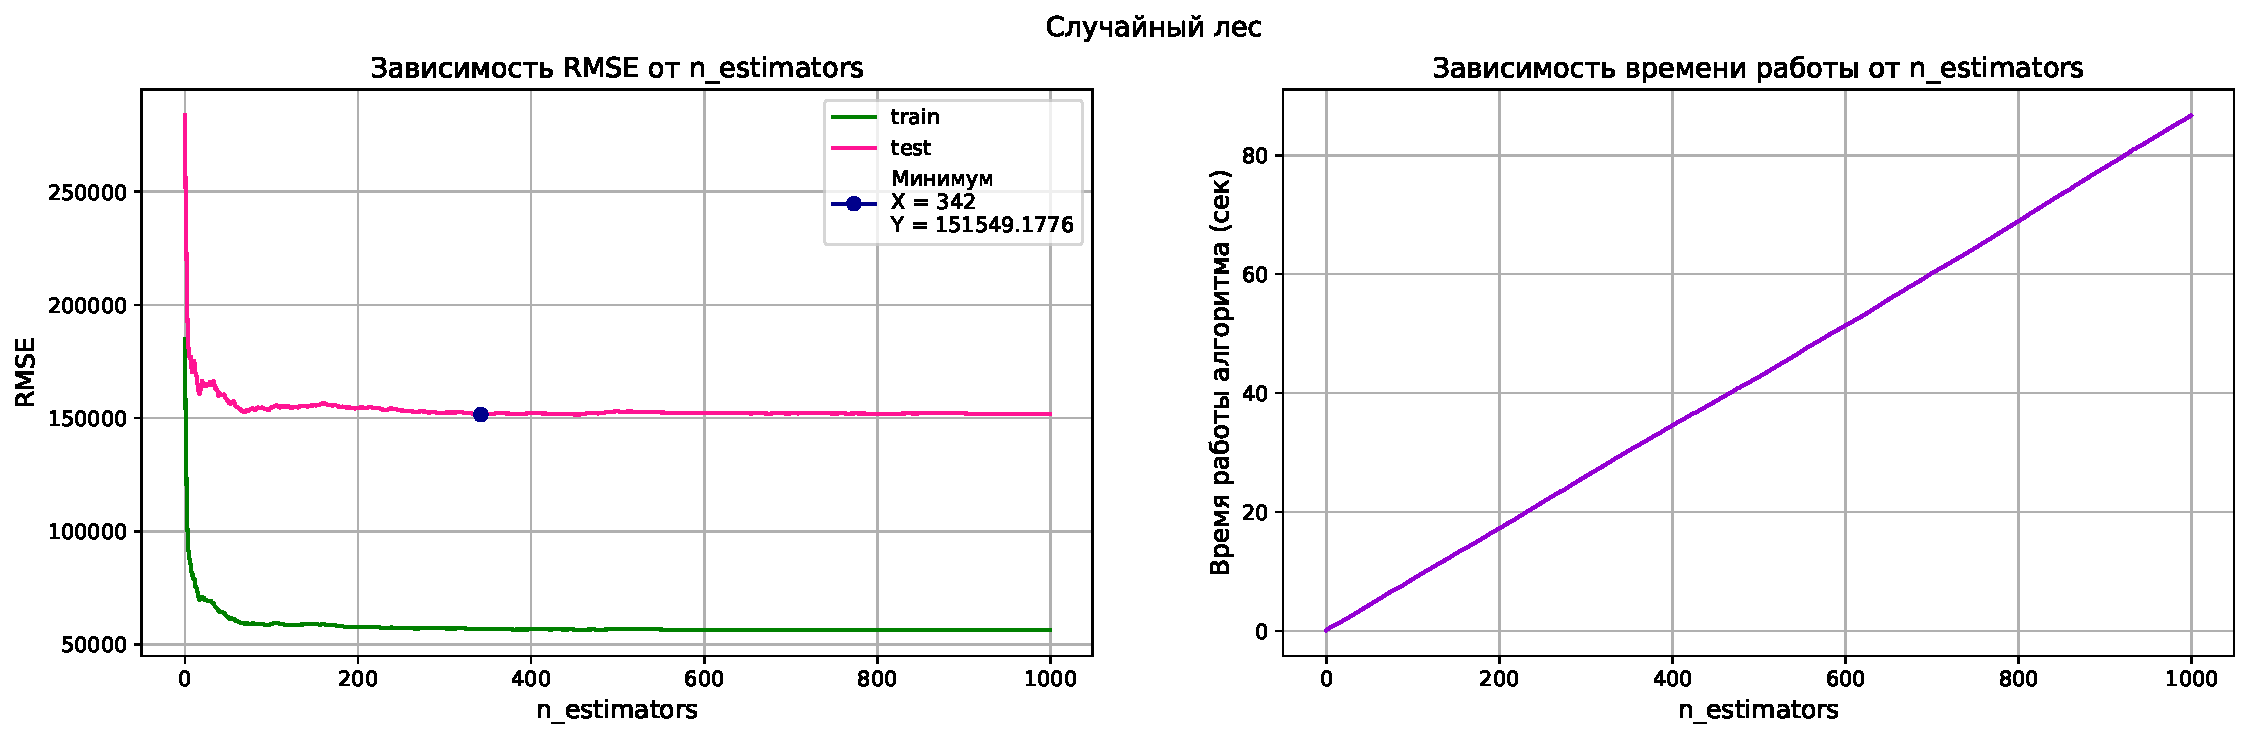
\includegraphics[scale=0.9, width=17cm]{S_1.pdf}
	\centering
	\caption{Зависимость RMSE и времени работы от количества деревьев в ансамбле (RF)}
	\label{pic:1}
\end{figure}

Параметр $n\_estimators$ в RF регулирует количество деревьев,  На графике \ref{pic:1} видно, что ошибка на обучающей выборке монотонно убывает. На валидации же немного возрастает при увеличении количества деревьев от $\sim350$, это свидетельствует о малом переобучении. Время обучения деревьев примерно одинаковое, поэтому было ожидаемо, что время обучения леса будет зависеть линейно от числа деревьев.

\end{subsubsection}

\begin{subsubsection}{2.2) Размерность подвыборки признаков для одного дерева}
\begin{figure}[H]
	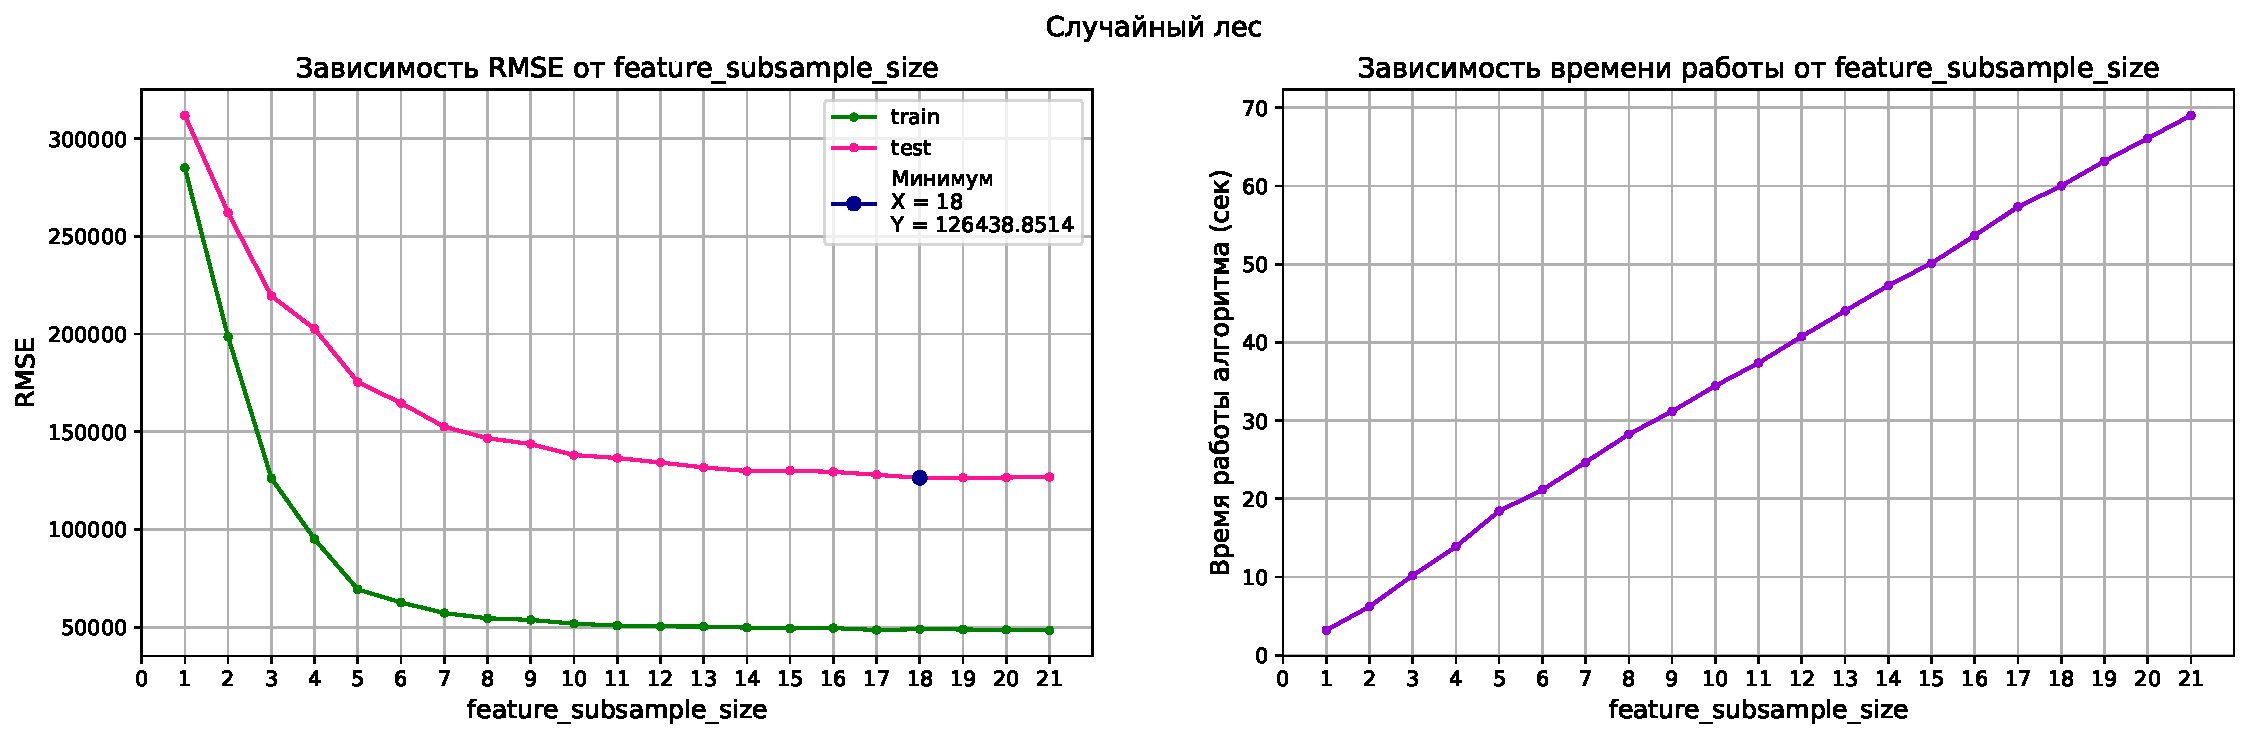
\includegraphics[scale=0.9, width=17cm]{S_2.pdf}
	\centering
	\caption{Зависимость RMSE и времени работы от размерности подвыборки признаков для одного дерева (RF)}
	\label{pic:2}
\end{figure}

Параметр $feature\_subsample\_size$ определяет по скольким признакам будет обучаться каждое дерево. Из графика \ref{pic:2} делаем вывод, что выгоднее всего будет взять почти все признаки. В данном случаем так же наблюдается линейная зависимость времени от числа признаков.


\end{subsubsection}

\begin{subsubsection}{2.3) Максимальная глубина дерева}
\begin{figure}[H]
	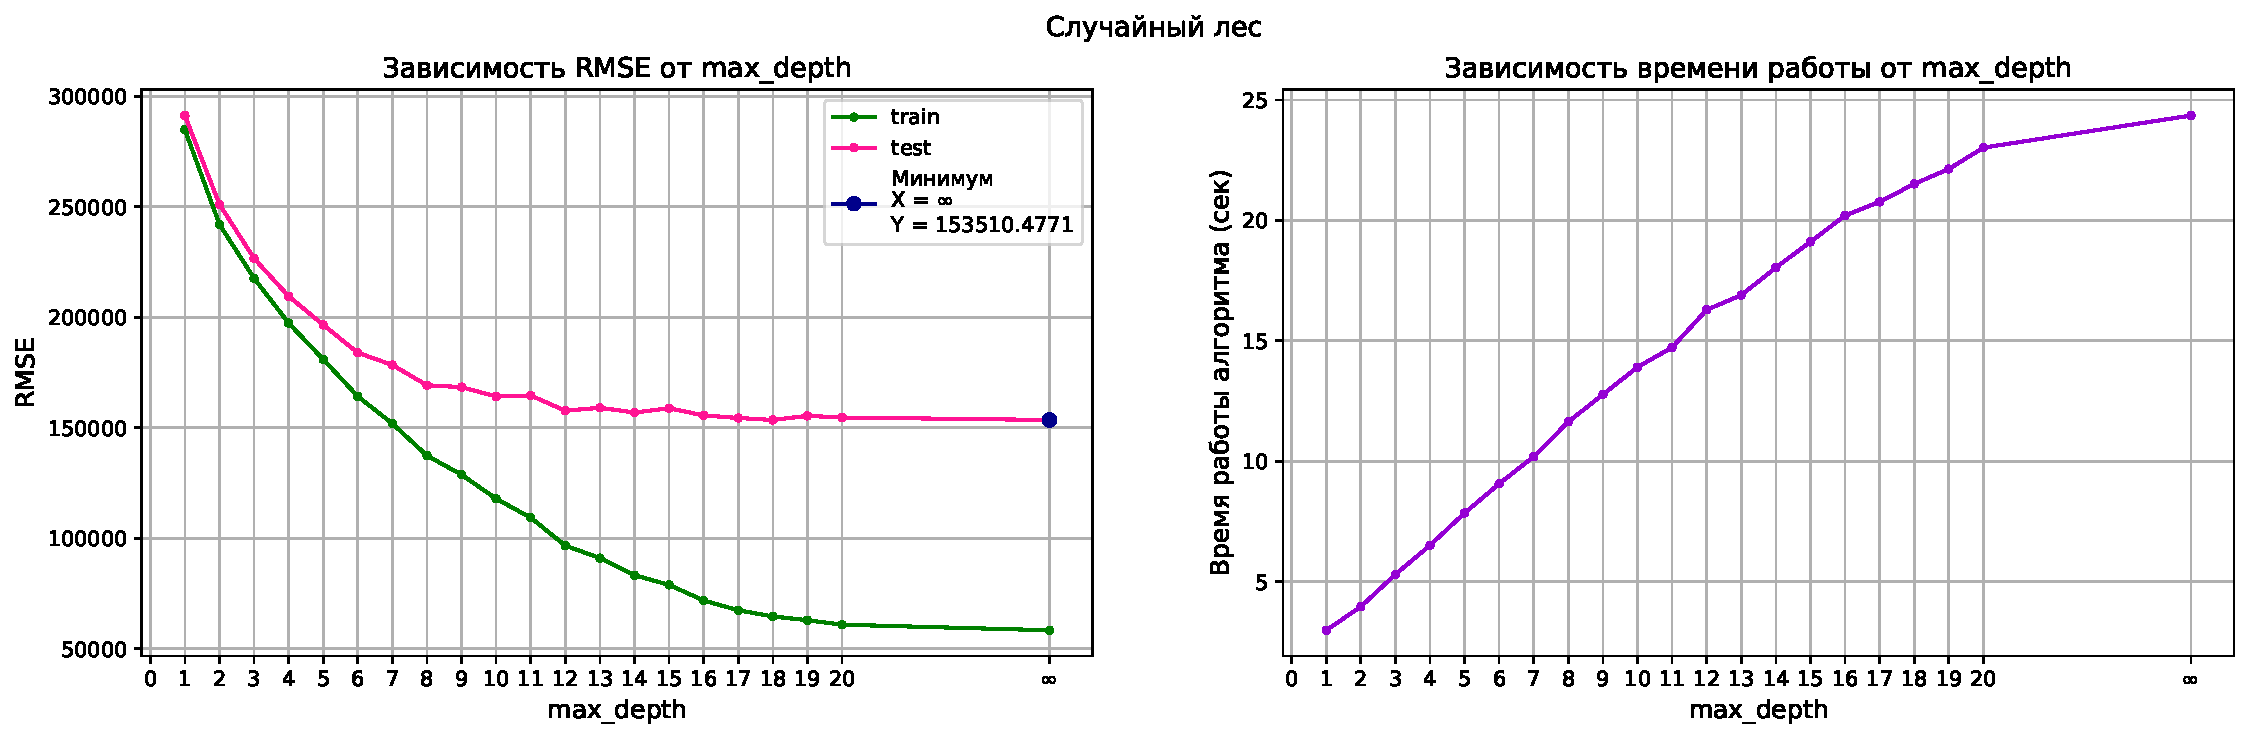
\includegraphics[scale=0.9, width=17cm]{S_3.pdf}
	\centering
	\caption{Зависимость RMSE и времени работы от максимальной глубины каждого дерева (RF)}
	\label{pic:3}
\end{figure}
Параметр $max\_depth$ определяет глубину каждого дерева в ансамбле. \par
В данном эксперименте отдельно рассматривался случай неограниченной глубины (он условно обозначается <<$\infty$>> на графике \ref{pic:3}).
Из теории мы знаем, что бэггинг лучше всего стоить на переобученных деревьях, что подтверждается нашим опытом. \par Скорее всего, использование деревьев неограниченной глубины было бы невыгодно по времени для большего признакового пространства или для большей обучающей выборки, но в нашем случае время увеличивается всего на 4-8\%. \par
Время возрастает чуть-чуть медленнее, чем линейно.
\end{subsubsection}

\end{subsection}

\begin{subsection}{3) Градиентный бустинг}

\begin{subsubsection}{3.1) Количество деревьев в ансамбле}
\begin{figure}[H]
	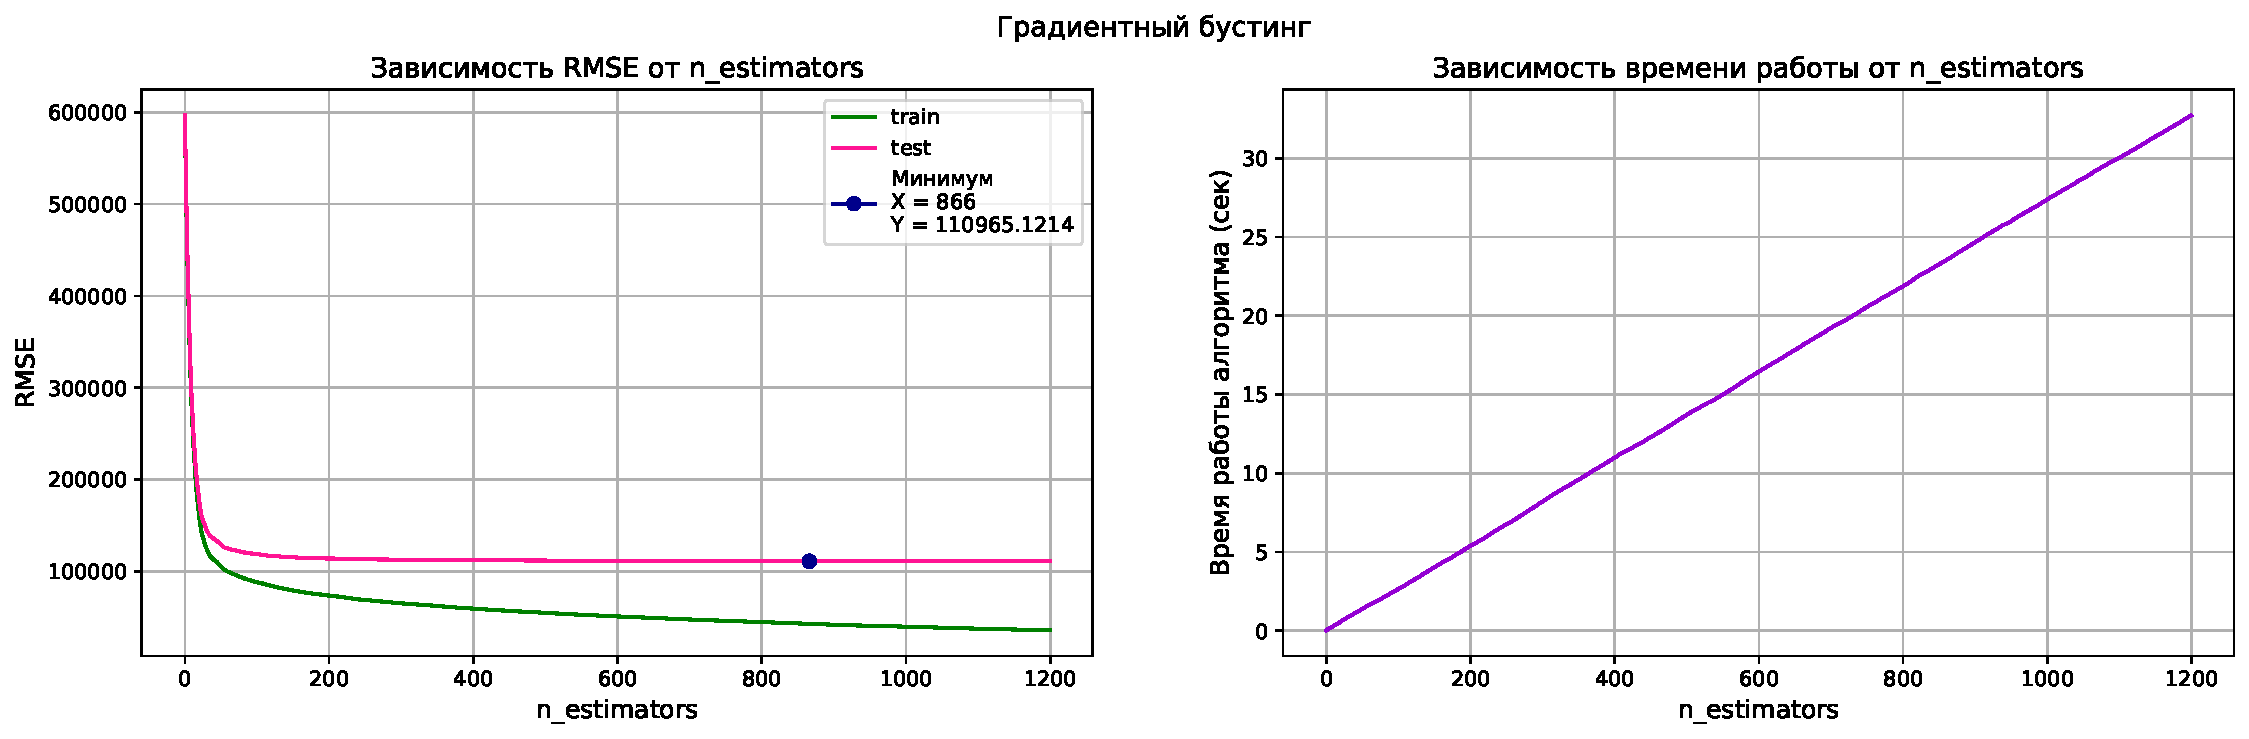
\includegraphics[scale=0.9, width=17cm]{G_1.pdf}
	\centering
	\caption{Зависимость RMSE и времени работы от количества деревьев в ансамбле (GB)}
	\label{pic:4}
\end{figure}
Как и в модели случайного леса на графике \ref{pic:4} видно, что ошибка на обучающей выборке монотонно убывает. На валидации же практически не видно переобучения при увеличении количества деревьев от $\sim850$. Из теории мы знаем, что бустинг переобучается только на громадном количестве деревьев, но такие эксперименты потребовали бы намного больше времени.\par Время обучения деревьев примерно одинаковое, поэтому было ожидаемо, что время обучения леса будет зависеть линейно от числа деревьев.

\end{subsubsection}

\begin{subsubsection}{3.2) Размерность подвыборки признаков для одного дерева}
\begin{figure}[H]
	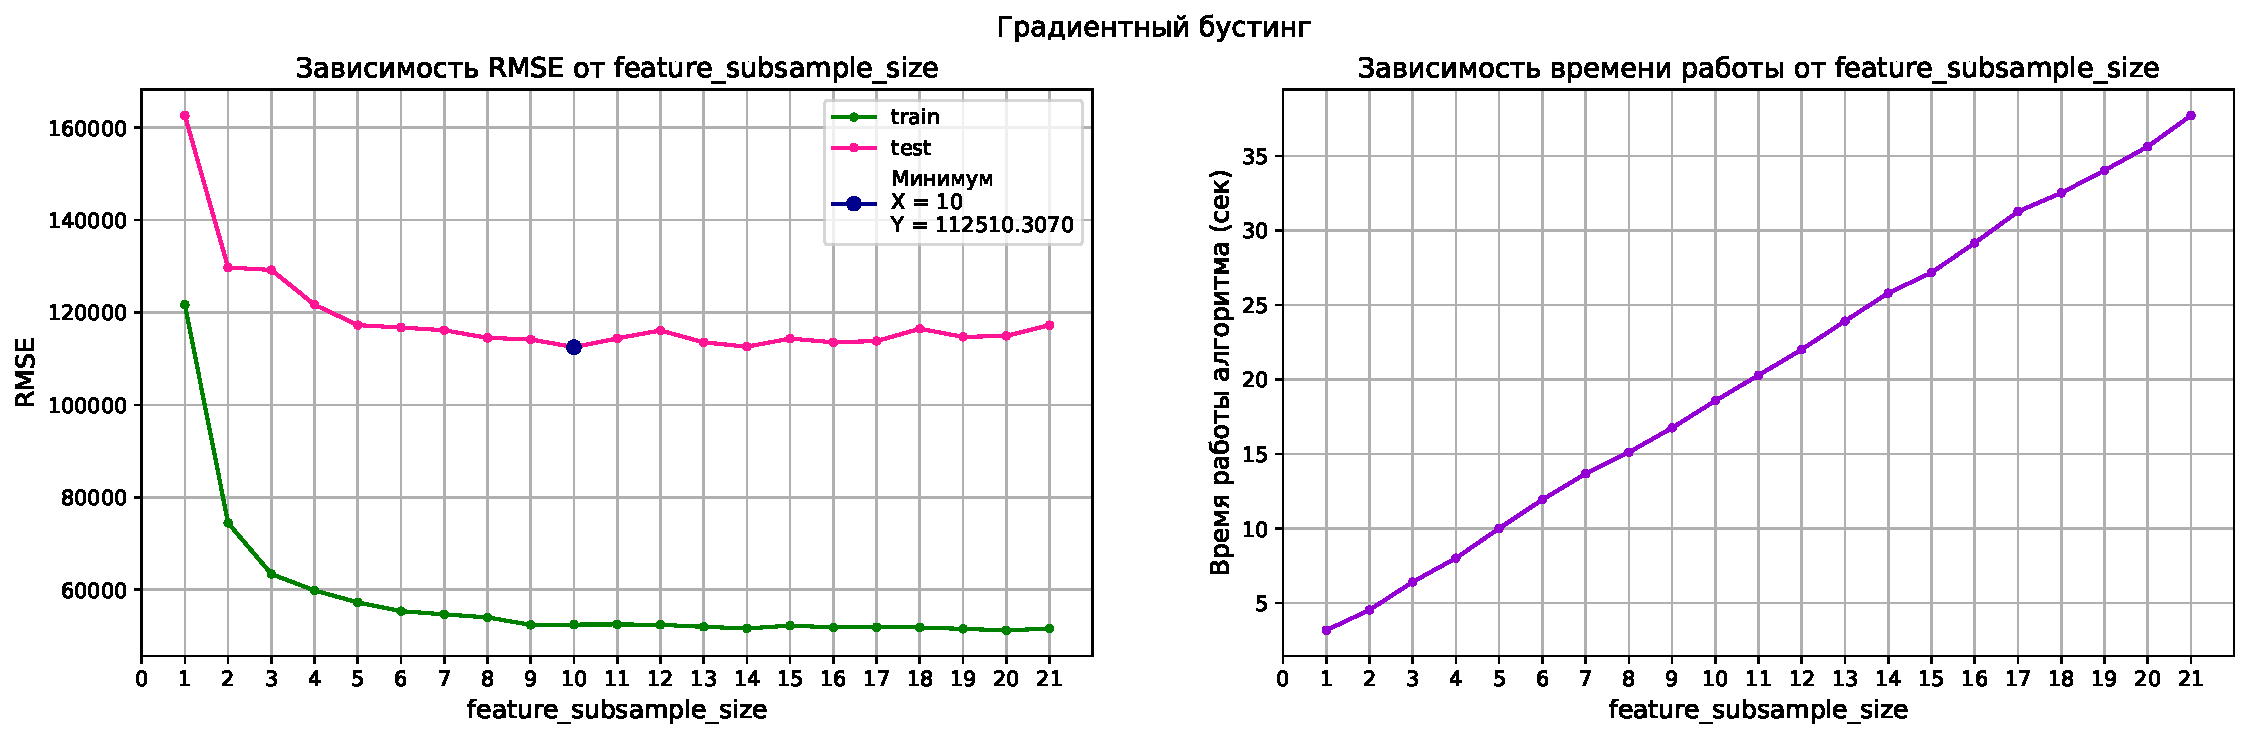
\includegraphics[scale=0.9, width=17cm]{G_2.pdf}
	\centering
	\caption{Зависимость RMSE и времени работы от размерности подвыборки признаков для одного дерева (GB)}
	\label{pic:5}
\end{figure}
Видно, что графики \ref{pic:2} и \ref{pic:5} имеют разное поведение. В случае градиентного бустинга нет стремления к какой-либо асимптоте, экстремум легко определяется <<на глаз>>. Зависимость времени так же линейная.
\end{subsubsection}

\begin{subsubsection}{3.3) Максимальная глубина дерева}
\begin{figure}[H]
	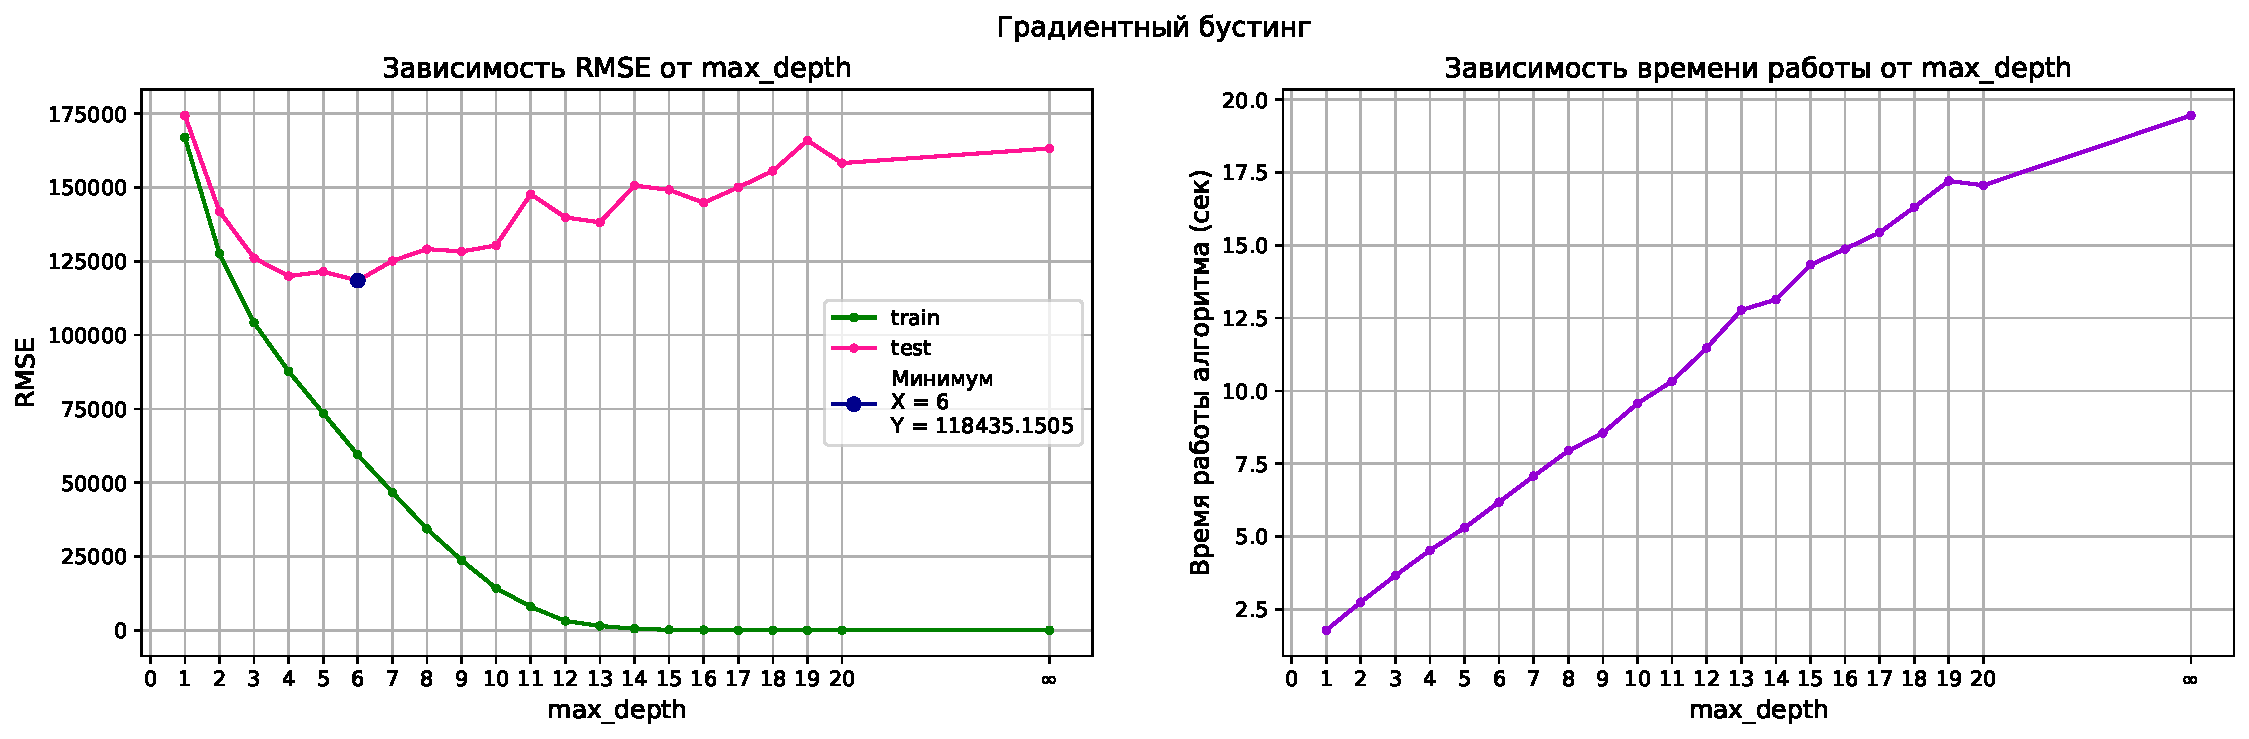
\includegraphics[scale=0.9, width=17cm]{G_3.pdf}
	\centering
	\caption{Зависимость RMSE и времени работы от максимальной глубины каждого дерева (GB)}
	\label{pic:6}
\end{figure}

В градиентном бустинге обучение обычно проводится на большом количестве неглубоких деревьев, что сочетается с результатами \ref{pic:4} и \ref{pic:6} экспериментов. При увеличении глубины бустинг очень сильно переобучается, ошибка на обучающем выборке стремится к нулю. \par 
Зависимость времени обучения тоже можно считать линейной, если не учитывать случай неограниченной глубины.
\end{subsubsection}

\begin{subsubsection}{3.4) Выбор темпа обучения}
\begin{figure}[H]
	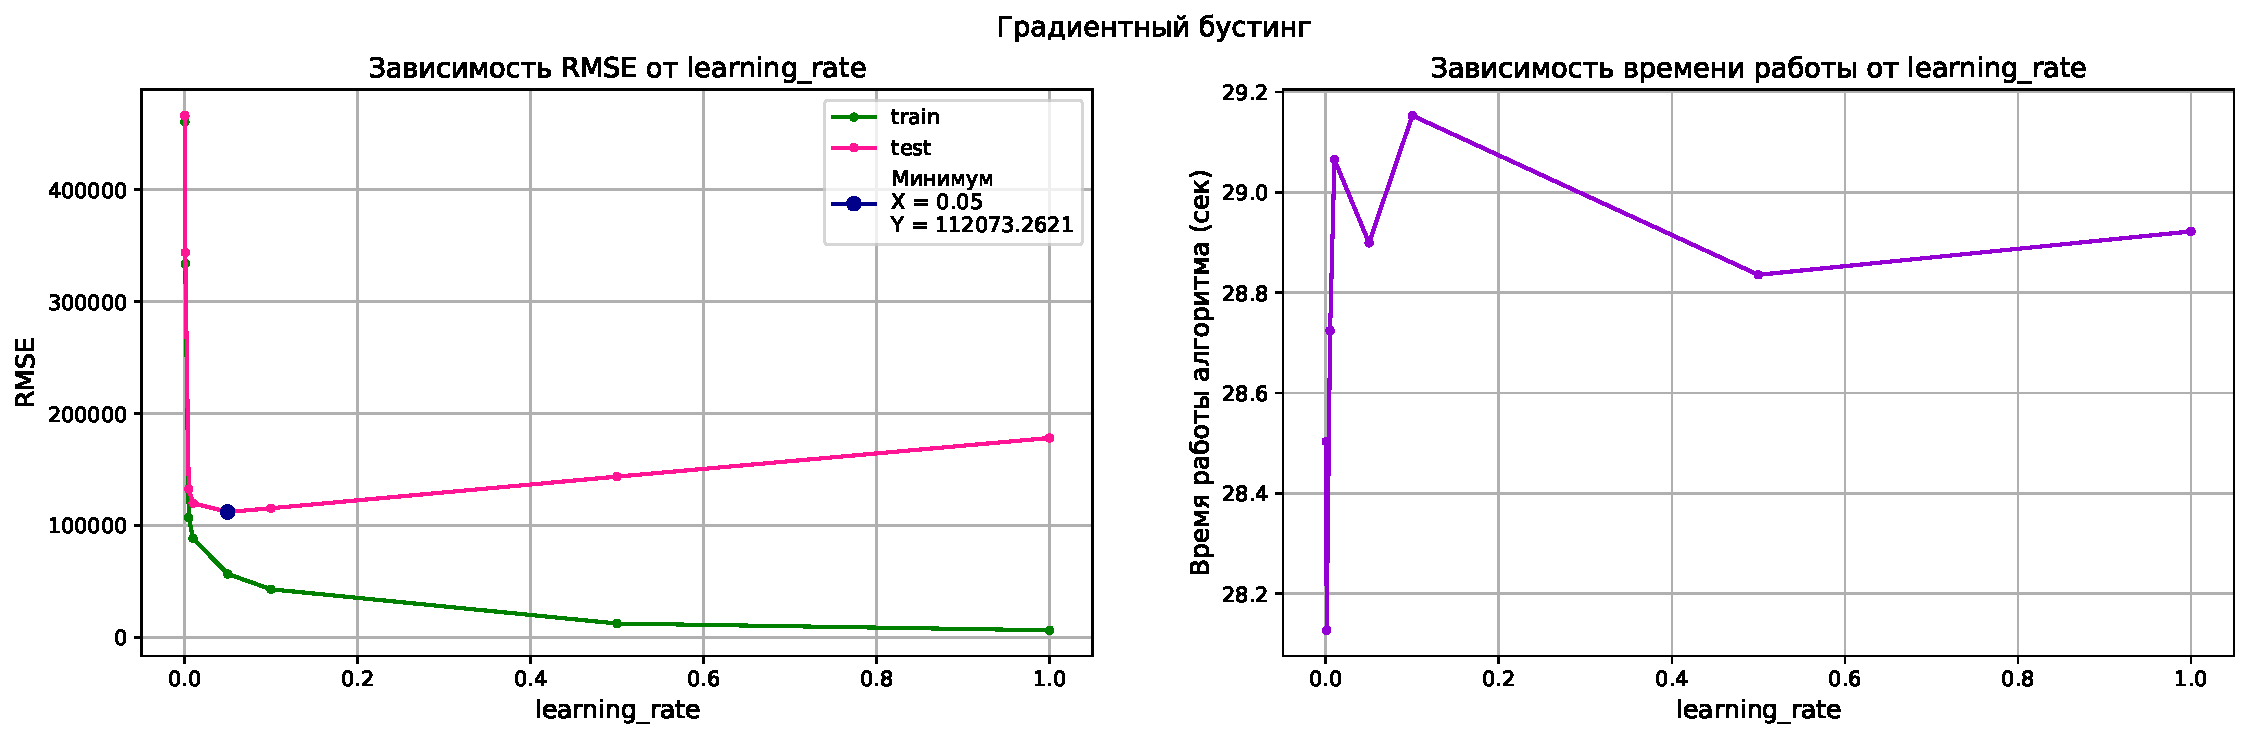
\includegraphics[scale=0.9, width=17cm]{G_4.pdf}
	\centering
	\caption{Зависимость RMSE и времени работы от темпа обучения (GB)}
	\label{pic:7}
\end{figure}
В методе градиентного бустинга каждое следующее дерево зависит от предыдущих, пытается <<исправить>> их ошибки. Темп обучения (параметр $learning\_rate$) определяет, насколько быстро меняются деревья. \par  
Из графика \ref{pic:7} видно, что от данного параметра больше всего зависит предсказание модели, на маленьких и больших значениях ошибка сильно возрастает. \par  Ранее по умолчанию использовалось значение $learning\_rate = 0.1$, что близко к оптимальному.

\end{subsubsection}

\end{subsection}

\begin{section}{Сравнение моделей}

\begin{table}[H]
	\begin{tabular}{c|c|c|c|c}
		Параметры & n\_estimators  & feature\_subsample\_size & max\_depth & learning\_rate     \\
		\hline
	    RF         & $ 350 $  & $  8 $   & $ $\infty$ $  & $ - $\\
		GB         & $ 850 $  & $ 10 $   & $ 6 $  & $ 0.05 $ \\
	\end{tabular}
	\centering
	\caption {Сравнение оптимальных параметров}
	\label{tbl:1}
\end{table}

\begin{table}[H]
	\begin{tabular}{c|c|c|c|c}
		Алгоритмы & RMSE на валидации  & Время (сек)   \\
		\hline
	    RF         & $ 153510.4771 $  & $  25 $   \\
		GB         & $ 112073,2621 $  & $ 6.75 $  \\
	\end{tabular}
	\centering
	\caption {Сравнение точности и времени}
	\label{tbl:2}
\end{table}

В заключение сравним ошибку и время работы на лучших параметрах. Из таблицы \ref{tbl:2} видим, что градиентный бустинг имеет меньшую ошибку, а по скорости превзошёл RF в несколько раз.
\end{section}


\end{section}

\begin{section}{Выводы}
И в начале исследований было понятно, что бустинг будет давать лучшие предсказания, так как каждая следующая модель становится <<лучше>> всех предыдущих. Но из проведённых экспериментов видно, что бустинг даёт лучшее предсказание и за меньшее время, что показывает его очевидноe превосходство над бэггингом.
\end{section}

\end{document}
